% ------------------------------------------------------------------------
% ------------------------------------------------------------------------
% ------------------------------------------------------------------------
%                                Capítulo 3
% ------------------------------------------------------------------------
% ------------------------------------------------------------------------
% ------------------------------------------------------------------------

\chapter{METODOLOGÍA PROPUESTA}

El enfoque propuesto de red neuronal profunda para la clasificación de objetos, a partir de medidas cuadráticas codificadas, incluye tres etapas principales: (i) capa de adquisición, (ii) enfoque de inicialización, (iii) y red de clasificación. La Figura \ref{fig:esquema_entrenamiento} ilustra el esquema de red neuronal profunda propuesto. Primero, una capa de adquisición simula el proceso de medición \eqref{eq:phase_retrieval_problem}, a través del modelado de la propagación del campo óptico. Luego, un procedimiento de inicialización aproxima el campo óptico $\mathbf{z}$. Finalmente, la red de clasificación infiere la clase correspondiente a cada medida cuadrática codificada.


\begin{figure}[!h]
    \centering
    \caption{Esquema propuesto de red neuronal profunda de tres etapas para la clasificación de objetos, a partir de medidas cuadráticas codificadas.}
    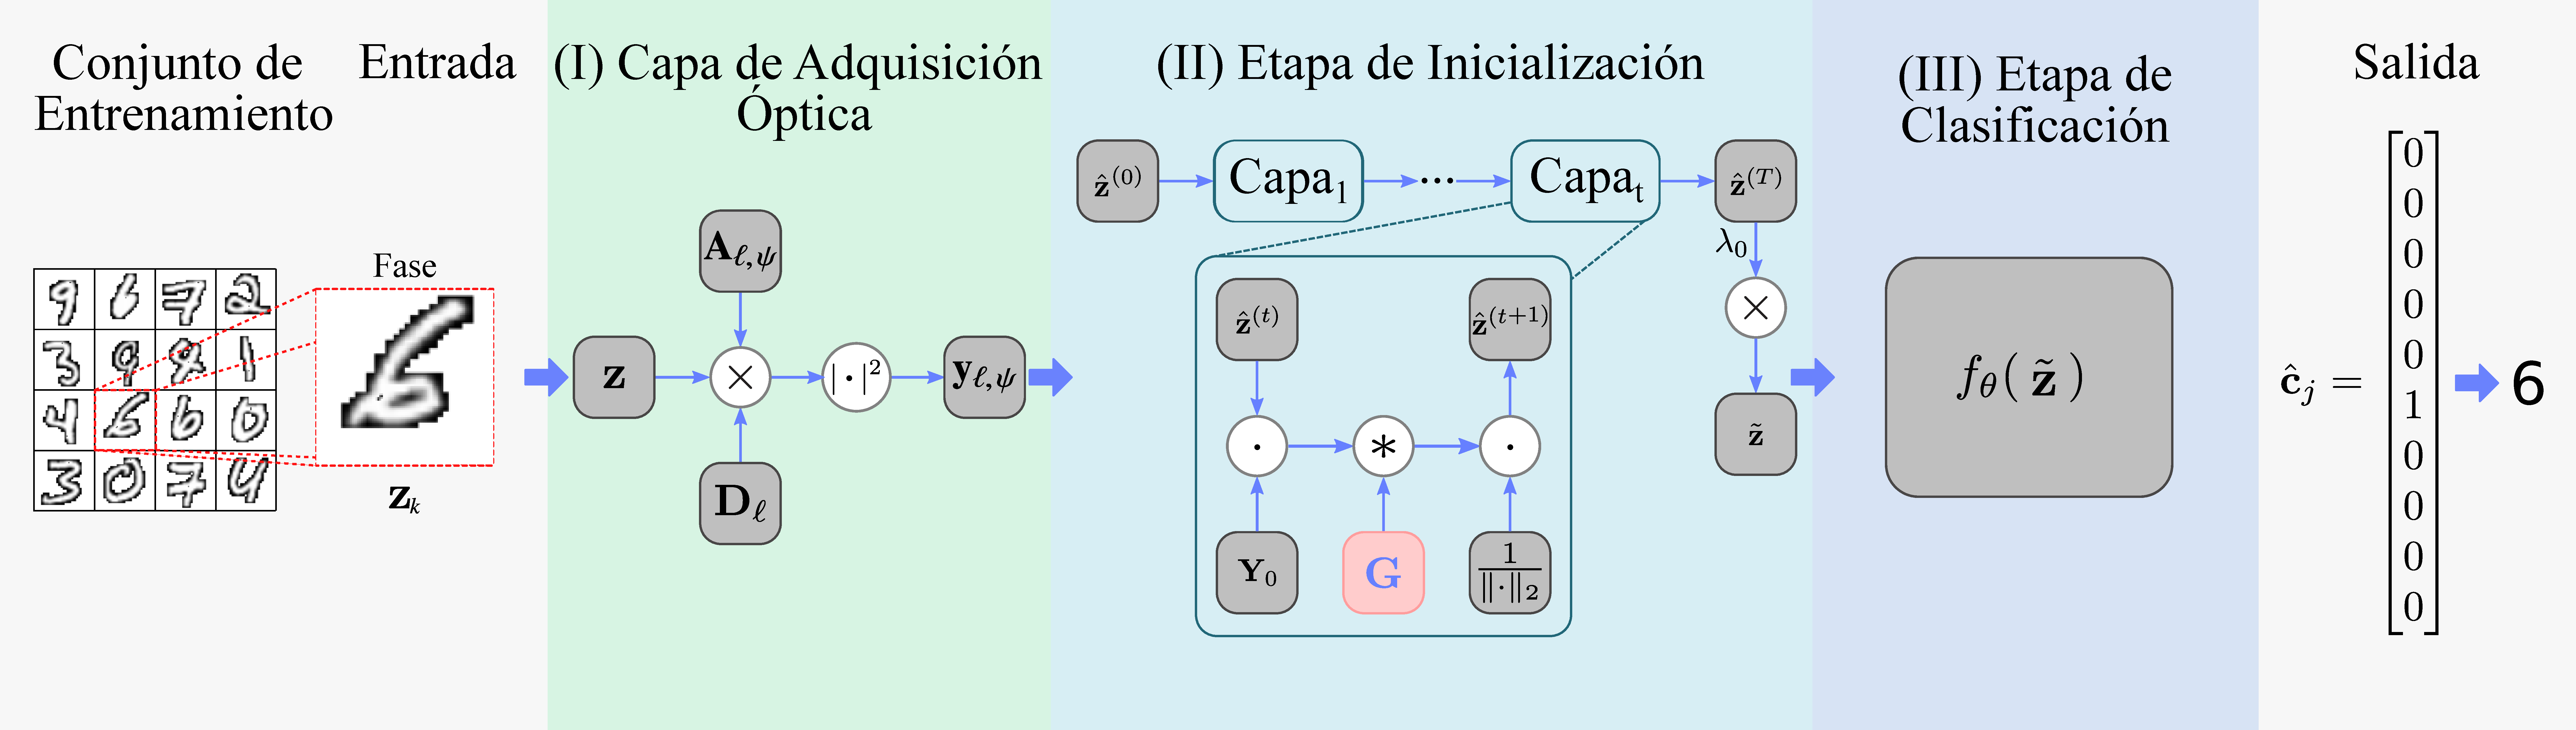
\includegraphics[width=\linewidth]{images/metodología/esquema_entrenamiento.pdf}
    \label{fig:esquema_entrenamiento}
\end{figure}


\section{ETAPA DE INICIALIZACIÓN}

En la etapa de inicialización del campo óptico, este trabajo aprovecha la matriz de adquisición $\mathbf{A}_{\ell, \psi}$ para crear un mapeo entre las medidas $\mathbf{y}_{\ell, \psi}$ y una aproximación más cercana del campo óptico $\mathbf{z}$, dada por el desenvolvimiento del algoritmo tradicional de inicialización de filtrado espectral \myfootcite{jerez2020fast} (FSI, de sus siglas en inglés \textit{filtered spectral initialization}), que incluye el aprendizaje de un filtro convolucional \myfootcite{Morales:22} (LFSI, de sus siglas en inglés \textit{learning filtered spectral initialization}), es decir que, $\hat{\mathbf{z}}=\mathrm{LFSI}(\mathbf{A}_{\ell, \psi}, \mathbf{y}_{\ell, \psi})$.

En concreto, este enfoque aplica un método iterativo para aproximar el campo óptico a partir de medidas cuadráticas codificadas, el cual se resume en el Algoritmo \ref{alg_1}. La aproximación dada por este algoritmo corresponde al cálculo de una versión filtrada de los mayores valores propios de la matriz
\begin{equation}
\mathbf{Y}_{0}:=\frac{1}{\mathrm{card}(\Xi)}\sum_{i\in\Xi}\frac{\mathbf{a}_{i,\psi}\mathbf{a}_{i,\psi}^\mathcal{H}}{\Vert\mathbf{a}_{i,\psi}\Vert_2^2},\label{eq:YO}
\end{equation}
donde $\mathbf{a}_{i,\psi}$ es la $i$-ésima columna de la matriz $\mathbf{A}=[\mathbf{A}_{1,\psi},\cdots,\mathbf{A}_{L,\psi}]^\mathcal{T}$, $\mathrm{card}(\cdot)$ es la cardinalidad del conjunto $\Xi$ correspondiente al conjunto de índices asignados a los valores más grandes de $\{(\mathbf{y})_i / \Vert \mathbf{a}_{i,\psi}\Vert_{2}\}$ con $\mathbf{y}=[\mathbf{y}_{1,\psi}^\mathcal{T},\cdots,\mathbf{y}_{L,\psi}^\mathcal{T}]^\mathcal{T}$.  Encontrar $\tilde{\mathbf{z}}$, teniendo en cuenta $\mathbf{Y}_0$ es posible resolviendo el siguiente problema de optimización


\begin{equation}
    \tilde{\mathbf{z}}=\argmax_{\Vert{\mathbf{z}}\Vert_2=1}{\mathbf{z}}^\mathcal{H}\mathbf{Y}_{0}{\mathbf{z}}.
\end{equation}


Tenga en cuenta que, la matriz $\mathbf{Y}_{0}$ se calcula en la línea 4 del Algoritmo \ref{alg_1}. En la línea 6, se aplica el filtrado mediante la operación de convolución $*$ entre $\mathbf{Y}_{0}\hat{\mathbf{z}}^{(t)}$ y en el kernel $\mathbf{G}$. Luego, la aproximación filtrada se normaliza en la línea 7. Finalmente, este algoritmo devuelve el vector complejo $\tilde{\mathbf{z}}$ en la línea 10, que se multiplica por el factor de escala $\lambda_0=\sqrt{\sum_{\ell=1}^{L}\frac{\Vert\mathbf{y}_{\ell,\psi}\Vert_{2}^2}{nL}}$ . %\textcolor{negro}{$\mathcal{O}(n\log n)$ }
  

Este trabajo propone la inicialización aprendida realizando un desenvolvimiento del algoritmo FSI en un esquema de red neuronal, como se muestra en la Figura \ref{fig:esquema_entrenamiento}. Adicionalmente, se incluye el filtro $\mathbf{G}$ como un parámetro entrenable de la red neuronal bajo una regularización definida a través de la siguiente función indicadora
\begin{equation}
  \mathcal{I}_{\Omega}(\mathbf{G})=  \left\{\begin{matrix}
 0& \text{si } \mathbf{G}\in \Omega \\ 
+\infty & \text{si } \mathbf{G}\notin \Omega 
\end{matrix}\right., \label{eq:regularizationG}
\end{equation}
donde $\Omega=\{\mathbf{G}\in\mathbb{C}^{g\times g}| |(\mathbf{G})_{p,q}|\leq 1\}$. 


\begin{algoritmo}[!h]
    %\scriptsize
    \caption{Algoritmo LFSI }\label{fsi_algo}
    \begin{algorithmic}[1]
        \State{\textbf{Entrada:} Matriz de sensado y muestras $\{(\mathbf{A}_{\ell,\psi};\mathbf{y}_{\ell,\psi})\}_{\ell=1}^L$, máximo número de iteraciones $T$, filtro $ \mathbf{G}\in\mathbb{C}^{g\times g}$.}
		\State{$\hat{\mathbf{z}}\leftarrow$ Escogido aleatoriamente.}
		\State{\textbf{Asignar }$\Xi$ como el conjunto de índices correspondientes a los valores más grandes de $\{(\mathbf{y})_i / \Vert \mathbf{a}_{i,\psi}\Vert_{2}\}$.}
		\State{$$\mathbf{Y}_{0}:=\frac{1}{\mathrm{card}(\Xi_0)}\sum_{i\in\Xi}\frac{\mathbf{a}_{i,\psi}\mathbf{a}_{i,\psi}^\mathcal{H}}{\Vert\mathbf{a}_{i,\psi}\Vert_2^2}$$}
		\For{$t=0:T-1$} 
		\State{$\grave{\mathbf{z}}^{(t+1)}= \mathbf{G}*\left(\mathbf{Y}_{0}\hat{\mathbf{z}}^{(t)}\right).$\Comment{Filtrado}}
		\State{$\hat{\mathbf{z}}^{(t+1)}=\frac{\grave{\mathbf{z}}^{(t+1)}}{\left \| \grave{\mathbf{z}}^{(t+1)} \right \|_2}$}.		\Comment{Normalización}
		\EndFor
		\State{Compute $\tilde{\mathbf{z}} = \lambda_0\hat{\mathbf{z}}^{(T)}$.\Comment{Escalado}}
		%		\State{Compute $\mathbf{z}_{1}=\mathcal{A}(\mathbf{z}_{0})$\Comment{Denoising step}}
		\State{\textbf{salida: } Estimación inicial del campo óptico $\tilde{\mathbf{z}}$.}
	\end{algorithmic}
    \label{alg_1}
\end{algoritmo}


\section{ETAPA DE CLASIFICACIÓN}

En este trabajo se propone un esquema de clasificación de medidas cuadráticas codificadas, que incluye una etapa de estimación inicial del campo óptico. De hecho, dentro del esquema de clasificación es posible emplear diferentes arquitecturas de clasificación previamente validadas en la literatura. Específicamente, se utilizaron tres arquitecturas de clasificación del estado del arte: MobilNetV2 \myfootcite{mobilnetv2}, InceptionV3 \myfootcite{inceptionv3}  y Xception \myfootcite{xception}. La Tabla \ref{tab:comp_class_models} resume el número de parámetros, la cantidad de capas de las redes neuronales de clasificación empleadas.

\begin{table}[!h]
\centering
\caption{Resumen de las arquitecturas de redes neuronales de clasificación utilizadas.}
\begin{tabular}{|c|c|c|}
\hline
\textbf{Modelo}      & \textbf{Número de parámetros} & \textbf{Número de capas} \\ \hline
MobileNetV2 & 3,538,984            & 53              \\ \hline
InceptionV3 & 23,851,784           & 48              \\ \hline
Xception    & 22,910,480           & 71              \\ \hline
\end{tabular}
\label{tab:comp_class_models}
\end{table}

El entrenamiento de los pesos $\theta$ de la red de clasificación $f_\theta(\cdot)$ se realizó mediante el siguiente problema de optimización

\begin{equation}
    \mathbf{\theta}^* \in  \argmin_{\mathbf{\theta}} \frac{1}{\mathcal{K}}\sum_{k = 1}^{\mathcal{K}} \mathcal{L}\left( c^{(k)}, f_\theta(\mathrm{LFSI}\left(\mathbf{A}_{\ell,\psi},\mathbf{y}_{\ell, \psi}\right)\right).
    \label{eq:dl_optimization}
\end{equation}

Este problema minimiza la función de pérdida, usualmente conocida como entropía categórica cruzada $\mathcal{L}(\cdot, \cdot)$, entre las etiquetas del conjunto de datos $c^{(k)}$ y las clases predichas $\hat{c}^{(k)} = f_\theta(\mathrm{LFSI}\left(\mathbf{A}_{\ell,\psi},\mathbf{y}_{\ell, \psi}\right))$, $\mathbf{y}_{\ell, \psi}^{(k)}$ es la medida cuadrática codificada del $k$-ésimo ejemplo y $\mathcal{K}$ es el número total de ejemplos del conjunto de datos.


\section{ESQUEMA PROPUESTO DE CLASIFICACIÓN DE OBJETOS}

El Algoritmo \ref{alg:algoritmo_2} resume el proceso de entrenamiento del esquema mostrado en la Figura \ref{fig:esquema_entrenamiento}. En primer lugar, en la línea 2 el filtro es inicializado usando una distribución uniforme $\mathcal{U}(\mathbf{0},\mathbf{1})$. Luego, el modelo de propagación descrito por \eqref{eq:phase_retrieval_problem} es simulado por la capa de adquisición en la línea 5. Posteriormente, en línea 6 se realiza el proceso de inicialización que aproxima el campo óptico inicial con base en las medidas cuadráticas codificadas obtenidas. En las líneas 7-9, el optimizador Adam $\mathcal{A}_{dam}(\cdot)$ se implementa para minimizar la función de pérdida \eqref{eq:dl_optimization} entre la clase etiquetada en el conjuto de datos ${\mathbf{c}}^{(k)}$ y la predicción $f_{\boldsymbol{\theta}}\left(\tilde{\mathbf{z}}^{(k)}\right)$. Esta función se minimiza sobre el filtro de la inicialización y los parámetros de la red neuronal de clasificación ponderados por $\beta_1$ y $\beta_2$, respectivamente. Finalmente, estos parámetros óptimos $\mathbf{G}$ y $\boldsymbol{\theta}$ se devuelven en la línea 12.


\begin{algoritmo}[!h]

        \caption{Enfoque de clasificación de objetos.}
            \label{alg:algoritmo_2}
        	\begin{algorithmic}[1]
            \State{\textbf{Entrada:} Conjunto de entrenamiento $\{\mathbf{z}^{(k)}, {\mathbf{c}}^{(k)}\}_{k=1}^\mathcal{K}$ con $\mathcal{K}$ imágenes.}  
            \State{\textbf{Inicialización filtro:} {\small
            $\mathbf{G}\in \mathcal{U}(\mathbf{0},\mathbf{1})^{5 \times 5}$} }
            \For{época = 1:$\mathcal{E}$}\Comment{$\mathcal{E}$ épocas}
                \For{$k= 1$:$\mathcal{K}$}\Comment{$\mathcal{K}$ ejemplos}
                    \State{$\mathbf{y}_{\ell,\psi} = \vert \mathbf{A}_{\ell,\psi}\mathbf{z}^{(k)}\vert^2, \quad \ell\in\{1,\dots,L\}$}
                    \Comment{Médidas cuadráticas codificadas}
                    \State{$\tilde{\mathbf{z}}^{(k)} \leftarrow  { \mathrm{LFSI}\left(\mathbf{A}_{\ell,\psi},\mathbf{y}_{\ell, \psi}\right)}$}\Comment{Algoritmo \ref{alg_1}}
                    %\State{$\hat{\mathbf{c}}^{(k)} \leftarrow  f_{\boldsymbol{\theta}}\left(\tilde{\mathbf{z}}^{(k)}\right)$}\Comment{Bloque de clasificación}
                    \State{$\mathcal{L}_{\mathbf{G},\boldsymbol{\theta}}=\frac{1}{\mathcal{K}}\sum_{k=1}^{\mathcal{K}} \mathcal{L}\left( c^{(k)},f_{\boldsymbol{\theta}}\left(\tilde{\mathbf{z}}^{(k)}\right) \right) $}    
               \Comment{Función de costo}     
                    \State{$\mathbf{G}\leftarrow\mathcal{A}_{dam}( \mathbf{G}, \beta_1 \nabla_{\mathbf{G}} \mathcal{L}_{\mathbf{G},\boldsymbol{\theta}}) $}    
                \Comment{Optimización sobre $\mathbf{G}$ }
                      \State{$\boldsymbol{\theta}\leftarrow\mathcal{A}_{dam}( \boldsymbol{\theta}, \beta_2 \nabla_{\boldsymbol{\theta}} \mathcal{L}_{\mathbf{G},\boldsymbol{\theta}}) $}    
                \Comment{Optimización sobre $\boldsymbol{\theta}$ }
                \EndFor
                \EndFor
		\State{\textbf{Salida: } Kernel óptimo $\mathbf{G}$ y parámetros de la red neuronal $\boldsymbol{\theta}$.}
	\end{algorithmic}
	%\label{alg:algoritmo_2}
\end{algoritmo}
